% Copyright 2021 Thomas Ascher
% SPDX-License-Identifier: CC-BY-SA-4.0

\documentclass[a4paper,parskip=half]{scrartcl}

\usepackage[T1]{fontenc}
\usepackage[ngerman]{babel}
\usepackage{csquotes}
\usepackage{chemformula}
\usepackage[regular,condensed,sfdefault]{roboto}
\usepackage{booktabs}
\usepackage{graphicx}
\usepackage{float}
\usepackage[style=apa,backend=biber]{biblatex}
\DeclareLanguageMapping{ngerman}{ngerman-apa}
\usepackage[hidelinks,pdfencoding=auto,
  pdfauthor={Thomas Ascher},
  pdfusetitle,
  pdfkeywords={Bier,Bierstil,Witbier}]{hyperref}
\usepackage{microtype}
\DisableLigatures{encoding=*, family=*}

\addto\extrasngerman{
\def\figureautorefname{Abb.}
\def\tableautorefname{Tab.}
\def\equationautorefname{Gl.}
}

\addto\captionsngerman{
\renewcommand{\figurename}{Abb.}
\renewcommand{\tablename}{Tab.}
}

\NewBibliographyString{gethesis}
\DefineBibliographyStrings{ngerman}{
  mathesis = {Masterarbeit},
  gethesis = {Diplomarbeit},
}

\title{Stilportrait: Witbier / Biere blanché}
\author{Thomas Ascher <thomas.ascher@gmx.at>}
\date{29. Dezember 2021, \href{http://creativecommons.org/licenses/by-sa/4.0/}{CC BY-SA 4.0}}

\addbibresource{witbier.bib}

\begin{document}
\maketitle

\section*{Kurzbeschreibung}

Bei Witbier handelt es sich um ein traditionelles belgisches, mit Gewürzen
aromatisiertes, weißliches und naturtrübes obergäriges Bier auf Weizenbasis, das
üblicherweise sehr kalt getrunken wird. \parencite[1\psq]{Strottner1999}
Die Celis Brauerei empfiehlt eine Trinktemperatur von circa 3,5 bis 5,5~°C
und die Verwendung eines oktagonalen Witbier-Glases \parencite{CelisBrewery2021}.

Typische Vertreter dieses Bierstils sind \parencite{Roncoroni2018}:

\begin{itemize}
\item Brugs – Brouwerij De Gouden Boom
\item Celis White – Brouwerij Van Steenberge
\item Hoegaarden – Brouwerij De Kluis
\item Watou's Wit – Leroy Breweries
\end{itemize}

\begin{figure}[h]
\centering
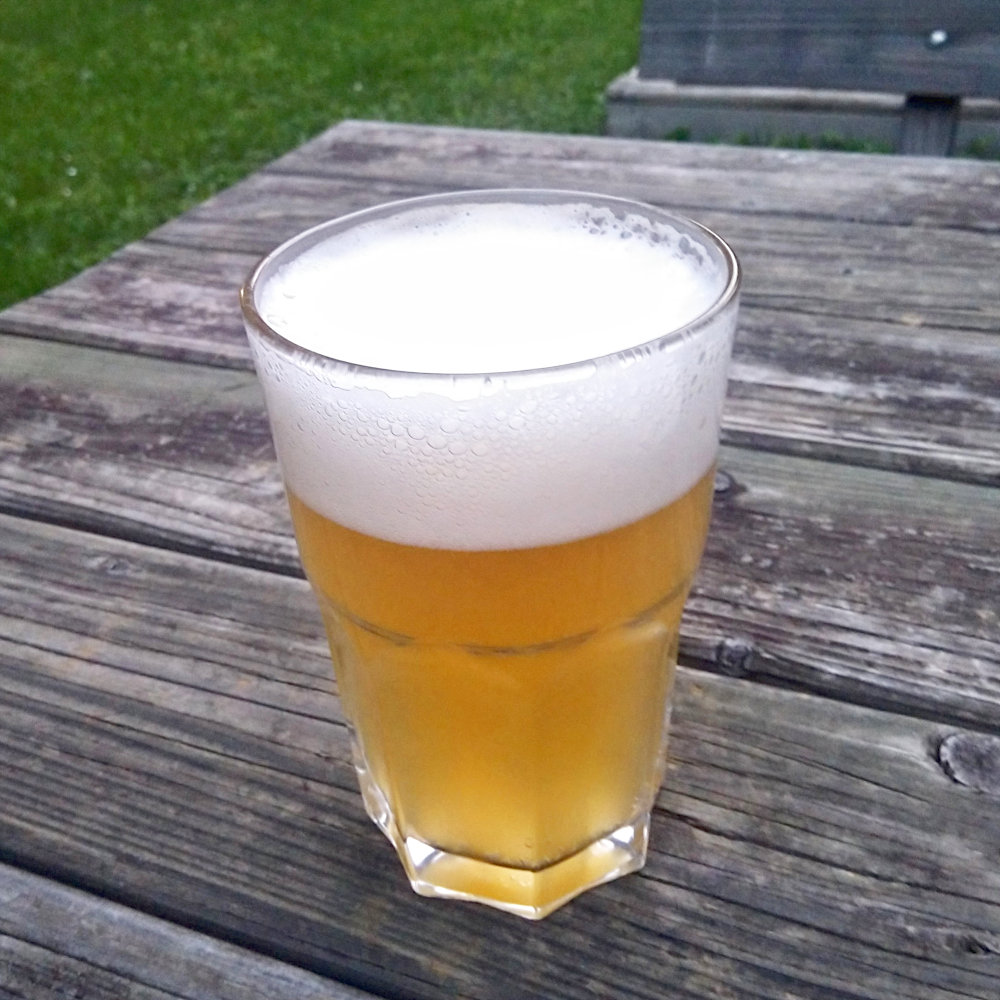
\includegraphics[width=4.8cm]{images/witbier.jpg}
\caption{Heimgebrautes Witbier (Ascher, 2021)}
\label{fig:witbier}
\end{figure}

\section*{Sensorischer Eindruck}

Die BJCP und die Brewers Association Stil-Richtlinien beschreiben
Witbier als ein leicht säuerliches Bier mit hoher Karbonisierung,
leichtem bis mittlerem Körper, geringen Malznoten, geringer Bittere
und kein bis geringes Hopfenaroma. Darüber hinaus sind hintergründige
Zitrusnoten sowie fruchtige Ester und phenolische Hefearomen (Gewürznelke)
vorhanden. Das Erscheinungsbild ist charakterisiert durch eine helle
bis leicht goldene Farbe, eine durch Stärke und Hefe induzierte Trübung
und einem dichten Schaum. \parencites[48\psq]{BJCP2015}[24]{BA2021}

\section*{Stilparameter}

In \autoref{table:parameters} sind die vom \citeauthor{BJCP2015} und die von
\citeauthor{Strottner1999} genannten brautechnischen Parameter erfasst.
Die Angaben der Brewers Association Stil-Richtlinien sind annähernd
deckungsgleich \parencites[24]{BA2021}. Einige am Markt erhältliche
Witbiere weisen allerdings nur einen gemessenen Bittergehalt von
2 bis 7~IBU auf \parencite{Roncoroni2018}.

\begin{table}[H]
\centering
\begin{tabular}{lrr}
\toprule
Parameter                    & \citeauthor{BJCP2015} & \citeauthor{Strottner1999} \\
\midrule
Alkoholgehalt [\%v/v]        & 4,5–5,5 & 4–6,9 \\
Stammwürze [°P]              & 11–12,9 & 9,4–14,9 \\
Scheinbarer Restextrakt [\%w/w] & 2,1–3,1 & 1,5–3,2 \\
Scheinbarer Vergärungsgrad [\%] & –       & 74,9–86,7 \\
Bittere [IBU]                & 8–20    & 9–18 \\
Farbe [EBC]                  & 4–8     & 6–14 \\
\bottomrule
\end{tabular}
\caption{Stilparameter \parencites[49]{BJCP2015}[23-113]{Strottner1999}}
\label{table:parameters}
\end{table}

Es existieren nur wenige Angaben hinsichtlich Karbonisierung.
\citeauthor{Zainasheff2007} nennt hierbei einen \ch{CO2} Gehalt von
4,9 bis 5,9~g/l bzw. 2,5 bis 3~vols \parencite{Zainasheff2007}.
Die BeerSmith Software empfiehlt sogar bis zu 6,7~g/l bzw. 3,4~vols.

\section*{Historische Entwicklung}

Der Ursprungsort des Witbiers ist das durch den Weizenanbau geprägte
Flämisch-Brabant im Zentrum von Belgien \parencite[44]{Roncoroni2018}.
Weitere Produktionsstandorte waren auch die Provinzen Hennegau und
Limburg \parencite[118]{Strottner1999}.
Belege dafür reichen zumindest bis in das 16. Jahrhundert
zurück, zu einer Zeit, als die kleine Stadt Hoegaarden größere
Teile des belgischen Biermarkts belieferte \parencite[46]{Mulder2020}. 
Durch gewährte Steuerprivilegien existierten dort zu Glanzzeiten 35
Brauereien auf nur 2000 Einwohner \parencite[27]{Sparrow2002}.

In Flämisch-Brabant wurde bereits ab dem Mittelalter Bier auf
Basis von Weizenrohfrucht gebraut. Damals aber noch mit
spontaner Gärung und Grut statt Hopfen zur Bitterung.
Besondere Bedeutung erlangten dabei die Witbiere aus Löwen
und aus dem 20 Kilometer entfernten Hoegaarden. In Löwen
entstand um 1425 eine Universität mit einer heute renommierten Brauschule
und im Jahr 1453 in Hoegaarden ein Kloster. Die dort ansässigen
Mönche haben später als Erste aromatisiertes Witbier mit
Curaçao Orangenschalen und Koriander gebraut. Flämisch-Brabant war
früher Teil der Niederlande. Durch den während der
Kolonialzeit vorherrschenden Gewürzhandel standen
Brauereien deshalb neue exotische Zutaten zur Verfügung.
\parencite[1,4]{Strottner1999}

Während des 17. und 18. Jahrhunderts war Witbier das beliebteste Bier
in der Stadt Brüssel \parencite{Zainasheff2007}.
Mehrere Umstände haben dann aber schlussendlich dazu geführt, dass
es für fast ein Jahrzehnt gänzlich vom Markt verschwunden ist.
Nach der Französischen Revolution den Brauereien in
Flämisch-Brabant gewährte Steuerprivilegien wieder entzogen
\parencite[44]{Roncoroni2018}. Während des Ersten Weltkrieges
musste dann aufgrund von Weizenrationierungen die Produktion gänzlich
eingestellt werden. Nach beiden Weltkriegen hat sich
das Konsumverhalten bedingt durch den amerikanischen
Einfluss zugunsten von untergärigen Bieren verschoben \parencite[4]{Strottner1999}. Letztendlich schloss im Jahr 1957 die letzte
Witbier produzierende Brauerei Tomsin ihre Tore \parencite[44]{Roncoroni2018}.

Der in den Fünfzigerjahren in Hoegaarden ansässige Milchhändler Pierre
Celis hatte gelegentlich bei Brauvorgängen bei Tomsin ausgeholfen. Im
Jahr 1966 begann er nach Beratung mit dem ehemaligen
Braumeister von Tomsin und der Gründung der Brauerei Celis
(später De Kluis) wieder mit der Produktion von Witbier. Die von
Celis geschaffene und von historischen Vorlagen abweichende Interpretation
gilt heute als Prototyp dieses Bierstils.
\parencite[37,49]{Hieronymus2010} 

Ab den frühen Achtzigerjahren erfährt der Konsum von Witbier – es
existieren mittlerweile mehrere produzierende Brauereien – national und
international einen starken Aufschwung. Allerdings war dieser
ab den Neunzigerjahren in Belgien selbst wieder rückläufig.
Celis selbst sieht sich im Jahr 1985 nach einem Feuer im Malzhaus der Brauerei
De Kluis dazu gezwungen, Unternehmensanteile an Artois (heute
AB InBev) zu veräußern. Nach dem Verkauf seiner restlichen Anteile
emigriert er in die USA und gründet dort die Brauerei Celis in Austin,
Texas. Nach mehreren Besitzerwechseln und dem Tod von Celis in 2011
hat dessen Tochter die Brauerei 2017 in Austin wiedereröffnet.
\parencites[1]{Strottner1999}[37,49]{Hieronymus2010}{Meewes2017}

Die Herstellungsmethoden und Zusammensetzung von Witbieren haben
sich über die Zeit zum Teil stark verändert und den heutigen
Marktanforderungen gerecht zu werden. Insgesamt wurden diese
Biere primär lokal ausgeschenkt und waren nur wenige
Wochen aufgrund der zunehmenden Säurebildung genießbar.
\parencite[118]{Strottner1999}

Historische Brauprozesse bestanden bis zu einundzwanzig
Einzelschritten mit sechs Teilmaischen und dauerten bis zu
17 Stunden. Dabei wurde oft nur ein geringer Endvergärungsgrad
von circa 50~\% erreicht. Durch eine geringe Nutzung von gealtertem
Hopfen, kurzen Kochzeiten, um helle Biere zu produzieren 
und geringe Anstellraten bei der Gärung waren die Biere besonders
anfällig für Infektionen durch Milchsäurebakterien und andere Mikroben.
Deshalb erfolgte eine Auslieferung an Kunden teilweise direkt nach
der Hauptgärung. Errungenschaften wie die Verwendung von
Hefereinkulturen statt spontaner Gärung und der Einsatz von
Kälteanlagen nach dem Ersten Weltkrieg haben die Produktionsbedingungen
nachträglich verbessert. \parencite[38-41]{Hieronymus2010}

Eine detaillierte Vorgehensweise für traditionelle Herstellungsprozessen
ist bei \citeauthor{Hieronymus2010}, \citeauthor{Mulder2020} und
\citeauthor{Strottner1999} beschrieben.

\section*{Schüttungszusammenstellung}

Extraktlieferanten für Witbier sind helle Gerstenmalze wie Pilsner Malz,
helle Weizenmalze, Zucker und Rohfrucht der Getreidearten Weizen, Roggen,
Dinkel, Hafer und Buchweizen \parencite[14]{Strottner1999}. Im 19.
Jahrhundert war der Einsatz von luftgetrocknetem Grünmalz gängig
\parencite[38]{Hieronymus2010}. \autoref{table:grains} zeigt die von \citeauthor{Strottner1999}
ermittelten Schüttungsanteile. Moderne Witbiere haben einen Weizenanteil
von 30 bis 50~\% \parencite[45]{Mulder2020}. Historische
Schüttungen weisen einen Haferanteil von bis zu 15~\% auf, wobei
einen Großteil davon auch Hafermalz bilden kann \parencite[45]{Hieronymus2010}.
Der Einsatz von Hafer ist optional. Die Hoegaarden Schüttung
besteht zum Beispiel aus 55~\% Gerstenmalz und 45~\% Weizenrohfrucht \parencite[43]{Strottner1999}.

\begin{table}[H]
\centering
\begin{tabular}{lr}
\toprule
Malz / Rohfrucht      & Anteil [\%] \\
\midrule
Gerstenmalz           & 50–60 \\
Weizenmalz            & 25–50 \\
Weizenrohfrucht       & 10–50 \\
Hafer (optional)      & 0,1–5 \\
Buchweizen (optional) & 0,1–5 \\
\bottomrule
\end{tabular}
\caption{Typische Schüttungsanteile \parencite[13]{Strottner1999}}
\label{table:grains}
\end{table}

Rohfrucht erfordert eine spezielle Behandlung bei der Maischeführung. Damit
die Stärke in der Rohfrucht für Enzyme zugänglich wird, muss diese zuerst,
abhängig von der Getreideart, für längere Zeit auf Verkleisterungstemperatur
gebracht werden. Es ist daher einfacher, den Rohfruchtanteil in der Schüttung
durch vorverkleisterte Weizen- und Haferflocken zu ersetzen.

% TODO Mosher, geschmackliche Veränderung

\section*{Maischeführung}

Die mehrstufige Infusion ist heute das meist verwendete Maischeverfahren
für Witbiere. \autoref{table:mashtable}
zeigt einen exemplarischen Rastverlauf. Die enthaltene
Eiweißrast dient zur Bildung von höhermolekularen Stickstoffsubstanzen die
Biertrübung begünstigten. \parencite[12,16]{Strottner1999}

\begin{table}[H]
\centering
\begin{tabular}{lrr}
\toprule
Rast              & Temperatur [°C] & Dauer [min] \\
\midrule
Einmaischen       & 38–56          & –     \\
Eiweißrast        & 50–56          & 10–35 \\
Maltoserast       & 60–64          & 20–60 \\
Verzuckerungsrast & 75             & –     \\
\bottomrule
\end{tabular}
\caption{Exemplarischer Rastverlauf \parencite[16]{Strottner1999}}
\label{table:mashtable}
\end{table}

Eine Zugabe von Rohfrucht erhört die Viskosität der Würze \parencite[9]{Strottner1999}.
Dadurch können Probleme beim Läutern entstehen, die durch Einsatz von
Reisspelzen gemindert werden können.

\section*{Hopfengaben}

Für Hopfengaben werden zumeist Aromahopfen in Form von Pallets
oder Dolden eingesetzt \parencite[1]{Strottner1999}. Passende
Sorten sind klassische europäische aber auch amerikanische
Hopfen wie Brewers Gold, Fuggles, Golding, Hallertauer Mittelfrüher,
Saazer, Spalter, Styrian Golding, Tettnanger und Target.
Witbiere sind weder besonders Bitter – 2 bis 20~IBU – noch
besonders hopfenaromatisch. Nach Meinung von \citeauthor{Zainasheff2007}
harmoniert das Hopfenaroma nicht besonders gut mit denen in einem Witbier
enthaltenen Gewürzen \parencite{Zainasheff2007}.

Das Hopfenkochen sollte kurz und schonend sein um den hohen Eiweißgehalt der
Würze beizubehalten. In der Praxis finden Kochdaueren von 30 bis 120
Minuten Anwendung. Es erfolgt dabei tendenziell nur eine Hopfengabe zu
Kochbeginn oder etwa 15 bis 30 Minuten vor Kochende. \parencite[13,17,23-113]{Strottner1999}

\section*{Gewürze}

Zur Aromatisierung eines Witbiers erfolgt eine Zugabe von getrockneten
Bitterorangenschalen (Curaçao Orangen) und Koriandersamen, aber auch
optional von weiteren Gewürzen wie zum Beispiel Holunderblüten,
Süßholz und Muskatnuss \parencite[1]{Strottner1999}. Modernere
Rezepturen enthalten auch Zitronenschalen \parencites[24]{BA2021}.

\citeauthor{Strottner1999} nennt eine Orangenschalenzugabe von
0,13 bis 0,8~g/l und eine Korianderzugabe
von 0,1 bis 0,5~g/l \parencite[13]{Strottner1999}.
Für ein klassisches Rezept ist eine Menge von 0,2~g/l Orangenschalen
und 0,25~g/l Koriander ausreichen \parencite[29]{Sparrow2002}.
Historische Witbiere enthielten eine geringere Koriandermenge
von nur 0,01 bis 0,02~g/l \parencite[40]{Hieronymus2010}.
Amerikanische Brauereien neigen tendenziell zu höheren
Gewürzgaben \parencite[26]{Strong2021}.

Koriander für die Bierherstellung sollte möglich frisch sein, da
dieser sonst Fehlaromen wie Sellerie und Seife anstatt der erwünschten
Zitrusnoten einbringen kann \parencite[26]{Strong2021}. Vor der Zugabe
sollte eine Zerkleinerung mit einem Mörser erfolgen \parencite[29]{Sparrow2002}. Nicht jede Koriander-Sorte ist für das Brauen geeignet. Ungeeignete
Sorten verursachen Schinken- oder Selleriegeschmack im Bier
\parencites[48]{BJCP2015}. \citeauthor{Mosher2015} empfiehlt die längliche
indische Sorte \parencite[338\psq]{Mosher2015}.

Um einen hohen Aromaverlust und eine adstringierende Bittere zu vermeiden,
sollte die Gewürze eher am Ende des Kochvorgangs für circa 15 Minuten
zugegeben werden. Alternativ kann auch ein Auszug nach dem Kochvorgang der
Würze zugegeben werden. Auch eine Zugabe während der Hauptgärung ist möglich,
birgt aber je nach Form ein Infektionsrisiko. \parencite[17\psq]{Strottner1999} 
Zur weiteren Reduktion des Infektionsrisikos gibt die Brauerei
Bavik die Gewürze bereits bei Kochbeginn hinzu und kompensiert den
Aromaverlust durch größere Gewürzmengen \parencite[62]{Hieronymus2010}.

\section*{Hefe}

Für die Gärung von Witbier kommen primär obergängige Hefestämme
zum Einsatz die zur Bildung des phenolischen Hefearomas
Gewürznelke (4-Vinyl Guaiacol) neigen \parencite[46]{Roncoroni2018}.
Hefen, die diesen Voraussetzungen entsprechen, sind
basierend auf Herstellerempfehlungen mit typischer Gärtemperatur,
in \autoref{table:yeasts} angeführt. Wyeast Hefen, die die
Bezeichnung PC bzw. „Private Collection“ in der Produktnummer enthalten,
werden nur gelegentlich aufgelegt. White Labs und Wyeast empfehlen
auch die Verwendung diverser Hefen für Saison- und Abteibiere,
die über ein passendes Aromaprofil verfügen.

\begin{table}[H]
\centering
\begin{tabular}{lllll}
\toprule
Hersteller      & Nummer  & Bezeichnung          & Form    & Gärtemp. [°C] \\
\midrule
Fermentis       & WB-06   & –                    & Trocken & 18–24        \\
Lallemand       & –       & WIT                  & Trocken & 17–22        \\
Mangrove Jack's & M21     & Belgian Wit          & Trocken & 18–25        \\
White Labs      & WLP400  & Belgian Wit          & Flüssig & 19–23        \\
White Labs      & WLP410  & Belgian Wit II       & Flüssig & 19–23        \\
Wyeast          & 3463 PC & Forbidden Fruit      & Flüssig & 17–25        \\
Wyeast          & 3942 PC & Belgian Wheat        & Flüssig & 18–23        \\
Wyeast          & 3944    & Belgian Witbier      & Flüssig & 17–25        \\
\bottomrule
\end{tabular}
\caption{Witbier Hefen verschiedener Hersteller (Ascher, 2021)}
\label{table:yeasts}
\end{table}

Nicht jedes mit Flaschengärung hergestellte Witbier eignet sich zum
Hefestripping. Manche Brauereien zentrifugieren die Hefe nach
der Hauptgärung ab und geben für die Flaschengärung eine
andere obergärige Staubhefe zu \parencite[43]{Strottner1999}.

\section*{Gärführung und Reifung}

Die Hauptgärung erfolgt in einem Temperaturbereich von 12 bis 25~°C
über einen Zeitraum von 3 bis 10 Tage \parencite[13,18]{Strottner1999}.
Der eine Temperatur unter 16~°C wird nur für das Anstellen verwendet.
Die Brauerei Bavik stellt zum Beispiel bei 18~°C mit 10 Millionen Zellen
per Milliliter bei einer Stammwürze von 11,5~°P an \parencite[63]{Hieronymus2010}.
Temperaturempfehlungen je Hefe sind \autoref{table:yeasts} zu entnehmen.
Es kann entweder über die gesamte Gärverlauf den gleiche Temperatur beibehalten
oder zunehmend erhört werden \parencite[63]{Hieronymus2010}.



\parencite[13]{Strottner1999}

Zucker als Speise

\parencite[14]{Strottner1999}
Warmlagerungsphase
22 bis 25°C
7 bis 18Tage
Kaltlagerungsphase
0 bis 2°C
7 bis 21 Tage

\parencite[39]{Hieronymus2010}
- trübung hoher Proteingehalt von Weizen und Wintergerste.
 Durch Bakterien. Getrunken während noch Hefe in schwebe war,
 typisch Staubhefen. Kartoffelstärke um Effekt zu verstärken

Bei mit Flaschengärung hergestellte Witbieren setzt sich über längere Zeit
die Teil der Eiweißtrübung mit der Hefe als Bodensatz ab.
\parencite[18]{Strottner1999}. 



 \parencite[18]{Strottner1999}.
Nach einer Speisezugabe vermischt man das Bier vorzugsweise
mit einer Staubhefe und lagert die Flaschen dann 7 bis 14 Tage bei 22 bis 25°C für
die Nachgärung.

Um den Geschmack der alten traditionellen Blanche besser zu treffen, fügen einige
Brauer dem Bier vor der Abfüllung Milchsäure und Essigsäure zu.

\section*{Brauwasseraufbereitung}

Sowohl weiches (3 bis 8~°dH) als auch hartes Wasser (20~°dH) findet
Anwendung bei der Witbier-Herstellung. Während des Maischevorgangs
wird der pH-Wert aber zumeist auf einen Wert zwischen 5,2 und
5,4 mit Milchsäure oder Phosphorsäure eingestellt. \parencite[14]{Strottner1999}

\section*{Rezept „Witgenstein“}

\url{https://braureka.de/rezepte/rezeptdetails/?id=38961}

Overall Brewhouse Yield (OBY) von 65~\%


\begin{table}[H]
\centering
\begin{tabular}{rl}
\toprule
\textbf{Ausschlagmenge} & 20~l \\
\textbf{Alkoholgehalt} & 5,1~\%v/v \\
\textbf{Stammwürze} & 11,8~°P \\
\textbf{Scheinb. Restextrakt} & 2,8~\%w/w \\
\textbf{Bittere} & 12~IBU \\
\textbf{Farbe} & 6~EBC \\
\textbf{Karbonisierung} & 5,8~g/l \\
\midrule
\textbf{Schüttung} & 2800~g Pilsner Malz (56~\%) \\
 & 1500~g Weizenflocken (30~\%) \\
 & 500~g Haferflocken (10~\%) \\ 
 & 200~g Reisspelzen (4~\%) \\
\midrule
\textbf{Wasser} & 20~l Hauptguss \\
 & 10,8~l Nachguss \\
\midrule
\textbf{Maische} & Einmaischen mit 52°C (50~°C) \\
pH-Wert 4,5 & Aufheizen auf 65°C, Rast 40~min \\
 & Aufheizen auf 78°C, Rast 10~min \\
\midrule
\textbf{Kochen} & 25~g Saazer Pellets (4,1~\%), 60~min \\
60~min & 30g Bitterorangenschalen, 10~min \\
 & 15g Koriandersamen, 10~min \\
\midrule
\textbf{Gärung} & 11~g LalBrew Wit, 18~°C, 7~Tage \\
\bottomrule
\end{tabular}
\end{table}

\printbibliography[title=Quellen]

\end{document}